\chapter{Eletricidade Cerebral}



\section{Correntes Elétricas}
%Gaspar, Alberto (2005). Física:Volume único. São Paulo: Editora Ática. 496 páginas. ISBN 9788508078837. Consultado em 12 de janeiro de 2012
A eletricidade é o nome dado a uma série de fenômenos que envolvem o fluxo de cargas elétricas (Gaspar, 2005). 
O potencial elétrico (também conhecido como tensão), é a quantidade de energia precisa para deslocar uma carga elétrica (Matias e Fratezzi, 2008). 
A diferença de potencial elétrico entre um material condutor gera um fluxo de 
cargas nomeado de \textbf{corrente elétrica} (Creder, 1989).
A intensidade do fluxo é medida em ampère (A) e determinada pela quantiadade de partículas que atravessam o seguimento
do condutor pelo tempo. As correntes podem ser contínuas ou alternadas, a depender se o sentido da corrente varia ou não; enquanto a corrente contínua 
é composta de polos, a alternada é composta de fases (Bhargava e Kulshreshtha, 1983). O calculo de corrente elétrica é 
dado pela seguinte equação:

\begin{equation}
    I = \frac{\Delta Q }{\Delta T},
\end{equation}

onde $\Delta Q$ é a quantidade de particulas que passam em um seguimento do condutor e $\Delta T$ indica o tempo. 

\section{Neurônios}
Os neurônios são células responsáveis pela condução de impulsos nervosos e se comportam como um “cabo eletrificado” - analogia
levantada a respeito da condução de impulsos elétricos, como apresentado no clássico estudo de Hodgkin e Huxley (1952), 
que teve como resultado uma modelagem dos potenciais de ação emitidos pelas células 
nervosas através de equações diferenciais não-lineares (figura 2.2). 
Os neurônios comunicam-se uns com os outros através das \textbf{sinapses}, onde ocorre a transmissão dos impulsos nervosos. 
É possível distinguir três partes anatomicas no neurônio: o corpo celular, o axônio e os dendrito (figura 2.1). 

\begin{figure}
    \centering
    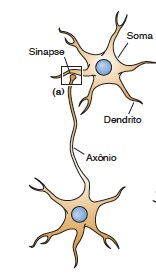
\includegraphics[width=40mm]{corpo_celular.jpg}
    \caption{Anatomia de um neurônio com destaque para área de sinapse entre neurônios. Fonte: Bear (2015)}
\end{figure}

% Serway, R.A.; Jewett Jr., J.W (2008). Princípios de Física. 3. São Paulo: Cengage Learning. p. 909-910. ISBN 85-221-0414-X
A membrana celular permite a passagem de cargas elétricas através de canais, que podem ou não necessitar de energia para a movimentação
das cargas. \textbf{Capacitores} são dispositivos de polaridades diferentes nas extremidades, que armazenam
cargas elétricas num campo elétrico (Serway, 2008). Por sua capacidade de separar cargas elétricas entre o ambiente interno e externo, 
a membrana celular age como os capacitadores, com sua capacitância (habilidade de armazenar cargas elétricas), definida pela seguinte equação:

\begin{equation}
    C = \frac{Q}{\Delta V},
\end{equation}

onde $C$ é a capacitância, $Q$ é a quantidade de carga armazenada e $\Delta V$ é a tensão elétrica, medida em farad (F). 
\textbf{Resistência elétrica} diz respeito a capacidade de oposição a passagem de corrente elétrica e é medido em
 ohms ($\Omega$). Os canais da membrana podem se comportar como resistores, se opondo a passagem da corrente elétrica, e sua 
 resistencia pode variar dependendo das condições celulares, como por exemplo se o canal está abero ou  não. Na figura 2.2, $E$ representa
 \textbf{bateria} pois a concentração de ions (particulas elétricas) é diferente no meio intra e extracelular, graças ao trabalho de canais ativos (com custo de energia
 para manter esse diferencial). De forma simplificada, a corrente aplicada no neurônio pode injetar corrente no capacitor e também 
 ser distribuída pelos canais. Dado a definição de um capacitor, $I_c = d u /d t$, é possível definir a corrente elétrica em uma seção da 
 membrana como:


%https://neuronaldynamics.epfl.ch/online/Ch2.S2.html#Ch2.F2
\begin{figure}
    \centering
    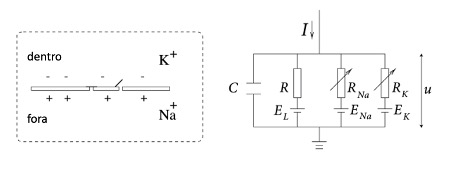
\includegraphics[width=100mm]{modeloHH.jpg}
    \caption{Esquema Modelo Hodgkin-Huxley. 
    Dentro: indicando espaço intracelular; fora: indicando espaço extracelular (imagem a esquerda). Direita: 
    C = capacitor, R = resistor, E = Baterias. Na = Sódio, K = Potássio  Fonte: Neuromal Dynamcs (2014)} 
\end{figure}

\begin{equation}
    C \frac{d u }{ d t} =  - \sum_{k} I_k (t) + I (t),
\end{equation}

onde $u$ = voltagem ao longo da membrana e $t$ = tempo. 




\subsection{Impulsos Nervosos e Potencial de Ação}
Para passar informações, os neurônios geram \textbf{impulsos nervosos}, ou alterações no potencial elétrico de sua membrana. Este sinal elétrico
ocorre quando o estímulo recebido pelo neurônio ultrapassa um limiar de ativação, que desencadeia uma série de respostas celulares. A célula pode 
estar em repouso (com valor do interior celular em cerca de -70mV), passando por despolarização (quando ocorre um fluxo de cargas elétricas que faz com 
que o meio intracelular passe a ser positivo em relação ao meio extracelular), e em repolarização, quando a célula está retornando ao potencial de repouso,
como representado na figura 2.3. 

O aumento do inicial da voltagem é causado pela entrada de sódio através de canais dependentes de voltagem, que se segue 
pela perda de potássio e fechamento dos canais de sódio. 


\begin{figure}[!h]
    \centering
    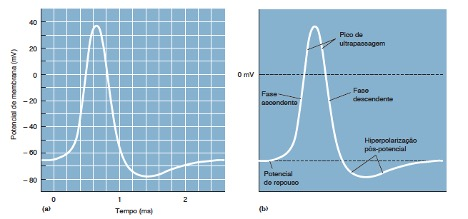
\includegraphics[width=120mm]{potencial_de_membrana_bear.jpg}
    \caption[Impulsos nervosos conduzidos em neurônios]{Resumo do potencial de ação. Fonte: Bear (2015).}.\label{fig:potencial}
    \end{figure}


\section{Eletroencefalograma}
O conjunto de impulsos nervosos de grupos de neurônios geram campos
magnéticos que podem ser captados por eletrodos colocados sobre a cabeça humana
(Kandel, 2000). Estes campos magnéticos foram primeiro registrados de coletas em
humanos aproximadamente em 1929, em um experimento conduzido pelo psiquiatra
alemão Hans Berger (Ince et al., 2021) – figura
2.4. Estes registros são o resultado dos potenciais de ação emitidos pelas células
nervosas abaixo do eletrodo, e permitem uma boa resolução temporal do
comportamento nervoso (podendo atingir precisão de milissegundos), mas em geral
não permitem uma boa resolução espacial (como identificar a localização espacial do
grupo celular responsável pela variação de voltagem observada).

  \begin{figure}[h]
    \centering
    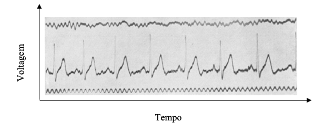
\includegraphics[width=100mm]{serie_temporal_EEG}
    \caption[]{Primeiro EEG registrado em humanos, resultado do trabalho do psiquiatra Hans Berger. Fonte: Ince et al. (2021).} 
    \end{figure}

\section{Ondas Cerebrais}
% Llinas, R. R. (2014). "Intrinsic electrical properties of mammalian neurons and CNS function: a historical perspective". Front Cell Neurosci. 8: 320. doi:10.3389/fncel.2014.00320. PMC 4219458free to read. PMID 25408634
O cérebro consegue gerar ondas ritmicas geradas pelos impulsos nervosos de grupos de neurônios. 
A oscilação de um neurônio único pode ser explorada na figura 2.3. As grandes oscilações (geradas por 
mais de um nerônio sendo ativado) pode ser detectada pelos eletrodos posicionados 
no crânio no eletroencefalograma (Llinas, 2014) e serem classificadas de acordo com suas características.
Um exemplo de agrupamento das ondas cerebrais pode ser observado na figura 2.5. 

\begin{figure}[h]
    \centering
    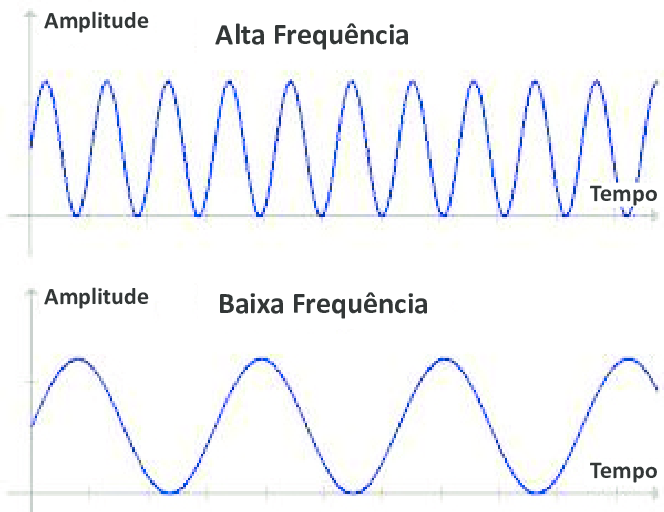
\includegraphics[width=100mm]{propriedades de onda.png}
    \caption[]{Representação das propriedades de onda.} 
    \end{figure}

As ondas cerebrais são caracterizadas pela \textbf{frequência, amplitude e fase} (figura 2.5). 
A amplitude mede a magnitude da oscilação de uma onda e pode ser representada pela equação

\begin{equation}
    y = A * sen (t - k) + b,
\end{equation}
onde $y$ é a função de onda (mede amplitude no instante t), $A$ é a amplitude da onda, sen representa
uma função senoidal, $t$ é o tempo, $k$ é a transalação temporal e b mede a translação de onda. 

\begin{figure}[h]
    \centering
    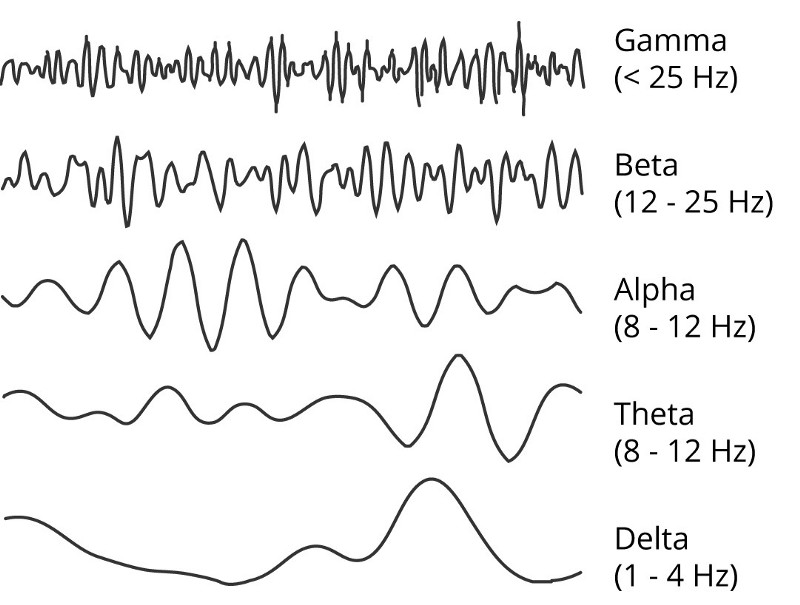
\includegraphics[width=80mm]{1_smvgacGqEOqIoKmjhzbfPw.jpeg}
    \caption[]{Ondas gamma, beta, alfa, teta e delta.} 
    \end{figure}


\subsection{Sistema Internacional 10/20 de Posicionamento de Eletrodos} 

    A técnica de registro de EEG vem sendo desde então aperfeiçoada e escolhida em
    investigações comportamentais devido a sua natureza não invasiva. Um exemplo de
    aperfeiçoamento foi a criação de um sistema internacional de posicionamentos de
    eletrodos para a coleta de EEG – o sistema 10/20 (Klem et al., 1999), 
    representado na figura 2.6.
    O registro capturado nos eletrodos
    advém de uma diferença de potencial elétrico. Esta diferença pode ser em referência à
    um eletrodo colocado em uma região externa ao escalpo (como orelha), ou à uma
    voltagem média comum (Tavares, 2011).


\begin{figure}[h]
    \centering
    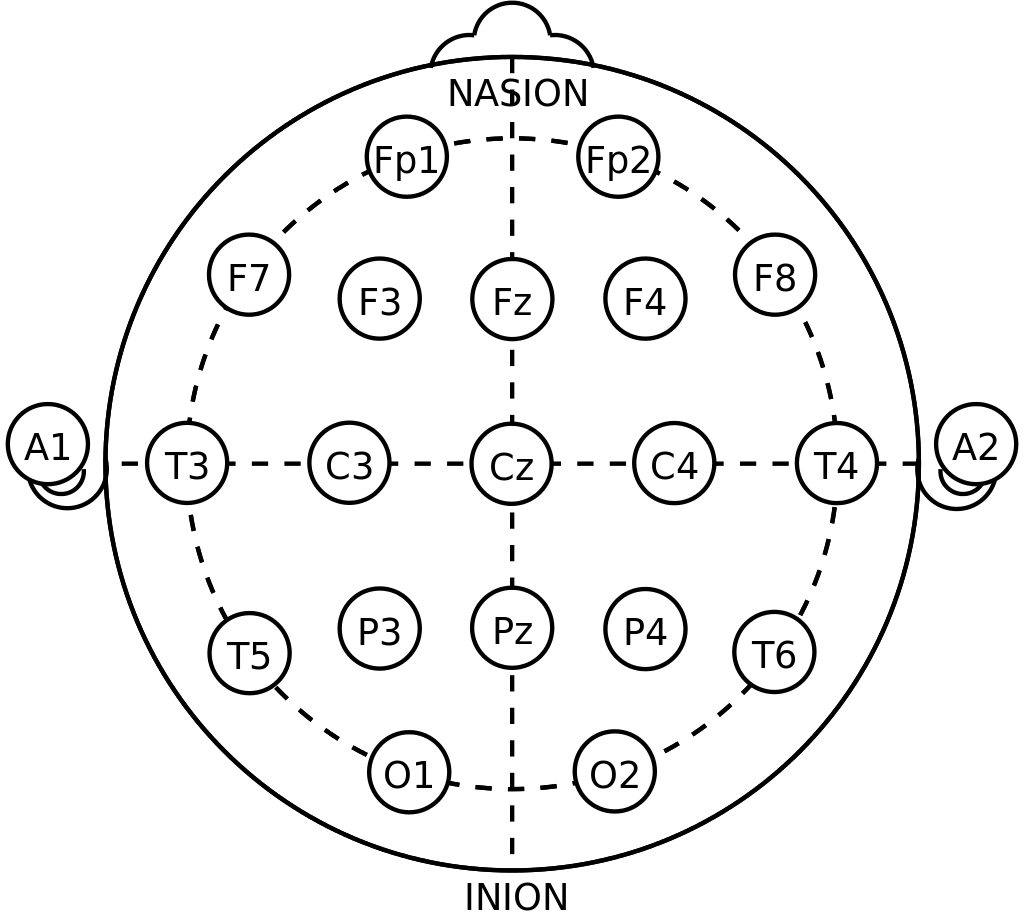
\includegraphics[width=100mm]{21_electrodes_of_International_10-20_system_for_EEG.png}
    \caption[]{Sistema Internacional 10/20 de Posicionamento de Eletrodos. Em destaque:
    Posição do eletrodo de coleta passiva do MindWave Mobile 2. A = Ear lobe, AF = anterior
    frontal, C = central, CP = centroparietal, F = frontal, FC = frontocentral, FT =
    frontotemporal, N = nasion, O = occipital, P = parietal, PO = parietooccipital, T = temporal.
    
    Klem et al. (1999).} 
    \end{figure}
    
    
        
\subsection{Tipos de Eletrodos para Captura de EEG}

    Existem diferentes tipos de eletrodos para a captura de EEG. 
    Um resumo é apresentado no quadro 2.1. É notável também que com o 
    desenvolvimento da capacidade computacional, novos recursos e métodos 
    para a análise destes dados vem sendo benéficos à construção do conhecimento 
    científico, agora também contando com o desenvolvimento de algoritmos de aprendizado
     de máquina, aprendizado profundo e inteligência artificial. 

     \begin{quadro}
        \caption{Tipos de Eletrodos para coleta de EEG (adaptado de Brain Support Inc. (2019)):}\label{quadro:exemplo}
        \begin{center}
        \scalefont{0.905}
        \begin{tabular}{|l|l|}
        \hline
        \hfill Tipo de Eletrodo\hfill\hspace{1mm} & \hfill Descrição\hfill\hspace{1mm}\\
        \hline
        Passivo &  \hspace{-06pt}\begin{tabular}{l}Geralmente feitos de prata, contam com a aplicação 
            de gel condutor \\
        para reduzir a perda de informação antes de serem colocados \\ na cabeça do participante.\end{tabular}\\
        \hline
        Ativo & \hspace{-06pt}\begin{tabular}{l}Geralmente feitos em prata, permitem o registro de \\
            variações de voltagem com redução de ruído do ambiente \\
            através de um circuito integrado aos eletrodos, com \\
            conversores de impedância.\end{tabular}\\
        \hline
        Seco & \hspace{-06pt}\begin{tabular}{l}Não necessita da aplicação de gel 
            para melhora da coleta do sinal.\end{tabular}\\
        \hline
        \end{tabular}
        \scalefont{1.4184}
        \end{center}
        \vspace{-12pt}
        Fonte: Brain Support Inc. (2019).\\
        \end{quadro}
        
  

    % Please add the following required packages to your document preamble:
% Please add the following required packages to your document preamble:
% \usepackage{graphicx}



%\subsection{Potenciais Relacionados a Eventos}


